\documentclass[10pt,twoside,spanish]{article}
%%%%%%%%%%%%%%%%%%%%%%%%%%%%%%%%%%%%%%%%%%%%%%%%%%%%%%%%%%%%%%%%%%%%%%%%%%%%%%%%%%%%%%%%%%%%%%%%%%%%%%%%%%%%%%%%%%%%%%%%%%%%%%%%%%%%%%%%%%%%%%%%%%%%%%%%%%%%%%%%%%%%%%%%%%%%%%%%%%%%%%%%%%%%%%%%%%%%%%%%%%%%%%%%%%%%%%%%%%%%%%%%%%%%%%%%%%%%%%%%%%%%%%%%%%%%
\usepackage[utf8]{inputenc}
\usepackage[spanish,english]{babel}
\usepackage[T1]{fontenc}
\usepackage{epsfig}
\usepackage{amsmath}
\usepackage{array}
\usepackage{amssymb}
\usepackage{epsf}
\usepackage{graphicx}
\usepackage{latexsym,bm}
\usepackage{amsthm}
\usepackage{amsfonts}
\usepackage{longtable}
\usepackage{multicol}
\usepackage{fancyhdr}
\usepackage{caption}
\usepackage[usenames]{color}
\usepackage[usenames]{colortbl}
\usepackage{setspace}
\usepackage{hyperref}
\usepackage{enumitem}

\setcounter{MaxMatrixCols}{10}

\newtheorem{theorem}{Teorema}[section]
\newtheorem{proposition}{Proposición}[section]
\newtheorem{lemma}{Lema}[section]
\newtheorem{corollary}{Corolario}[section]
\newtheorem{definition}{Definición}[section]
\newtheorem{remark}{Observación}[section]
\newtheorem{example}{Ejemplo}[section]
\newtheorem{conclusion}{Conclusión}[section]
\newtheorem{conjecture}{Conjetura}[section]
\newtheorem{notation}{Notación}[section]
\newtheorem{exercise}{Ejercicio}[section]
\newtheorem{problem}{Problema}[section]
\renewenvironment*{proof}[1][Demostración]{\noindent \textbf{#1.} }{\ \rule{0.5em}{0.5em}}
\numberwithin{equation}{section}
\renewcommand{\theequation}{\thesection.\arabic{equation}}
\renewcommand{\thefigure}{\arabic{figure}}

\font\gotica=eufm9 scaled\magstep2 \font\gotsmall=eufm8

\renewcommand{\baselinestretch}{1.1}
\footnotesep 0.2cm \skip\footins 0.3cm
\abovecaptionskip 0.2cm
\belowcaptionskip 0cm
\renewcommand*{\refname}{Referencias}
%\hyphenation{con-ve-nien-te te-o-re-mas}

\begin{document}

\title{%
\vspace*{-2cm}
\textbf{Bringing R to non-expert users with the package RKTeaching} 
%
%\thanks{}
\vspace*{-0.2cm}%
}
\author{Alfredo Sánchez Alberca\\
Departamento de Matemática Aplicada y Estadística \\
Universidad CEU San Pablo\\
asalber@ceu.es}
\date{}
\maketitle

\begin{abstract}
This article presents  a new package for R named RKTeaching, developed at the San Pablo CEU University to facilitate the learning of
Statistic for students of Health Sciences. This package is based on the graphical interface RKWard and has been designed to free students of
the technical and programming skills required to manage R, and to be as simple and intuitive as possible. The package helps students to
choose the most appropiate statistical test or procedure in many cases and to interpret the results correctly. After five years using this
package in the practical classes the assessment by the students clearly reflects its ease of use and learning compared to SPSS.
\medskip

\noindent\textbf{Keywords:} Statistic, Teaching, R, RKTeaching

\noindent\textbf{AMS Subject classifications: 97K80, 62P10, 90C90}

\end{abstract}

\selectlanguage{spanish}

\section{Introducción}
No cabe duda de que el soporte informático al análisis de datos ha supuesto una revolución en la Estadística Aplicada.
En las últimas décadas se ha desarrollado multitud de software específico para el análisis de datos, que ha impulsado la aplicación de la
Estadística a todas las áreas de las Ciencias Experimentales de una manera generalizada.
Este software ha permitido que, incluso profesionales no expertos en Estadística, puedan aplicar procedimientos estadísticos en sus análisis
de datos e investigaciones de manera sencilla.
De este modo, la docencia de la Estadística en nuestros días, ineludiblemente, va acompañada de la enseñanza del manejo
de algún programa de análisis de datos que permita a los usuarios abstraerse de los tediosos cálculos y centrarse en el análisis de los resultados.

En la última década, en la  Universidad CEU San Pablo se han utilizado programas de análisis de datos como
Excel\footnote{\url{http://office.microsoft.com/es-es/excel/}}, Statgraphics\footnote{\url{http://www.statgraphics.net/}} o
SPSS\footnote{\url{http://www-01.ibm.com/software/es/analytics/spss/}} para la docencia de la Estadística en titulaciones de Ciencias de la
Salud como Medicina, Farmacia, Psicología, Fisioterapia, Enfermería, Óptica y Nutrición. 
Estos programas tienen distintas ventajas e inconvenientes:
\begin{description}
\item[Excel] es posiblemente el programa más conocido y extendido por ir integrado en el paquete Office de Microsoft. Resulta
bastante fácil de manejar para análisis de datos sencillos, pero no incorpora procedimientos para análisis más complejos.
\item[ Statgraphics] es un programa bastante pedagógico relativamente fácil de aprender a usar, por lo que está muy extendido en el ámbito
universitario, pero muy poco en el ámbito hospitalario.
\item[SPSS] es posiblemente el programa más extendido en el ámbito hospitalario y en general en las ciencias biosanitarias por su potencia
para realizar casi cualquier tipo de análisis, ya que incorpora su propio lenguaje de programación. 
Su contrapartida es que tiene una mayor dificultad de aprendizaje.
\end{description}
Sin embargo, todos estos programas tienen el serio inconveniente de que no son software libre, lo que supone, en primer lugar, que hay que
pagar por su uso, lo que es un serio inconveniente para que los alumnos puedan acceder a ellos para  uso doméstico, sobre todo SPSS que
tiene un precio prohibitivo para pequeños usuarios.
Y en segundo lugar, no permiten acceder al código fuente, por lo que no son fácilmente adaptables a las necesidades docentes.

Por tal motivo, en el 2008 el departamento de Matemática Aplicada y Estadística de la Universidad CEU San Pablo se
planteó la introducción del software libre en la enseñanza de la Estadística.
En aquella época, el software libre de análisis de datos más extendido y con más proyección era R\footnote{\url{http://www.r-project.org/}}
[R Development Core Team (2001)] por lo que se decidió empezar a usarlo en las clases prácticas de Estadística de las titulaciones de
Farmacia y Medicina.

R es una implementación de código abierto del lenguaje de análisis de datos S.
Al ser, en el fondo, un lenguaje de programación especialmente pensado para el tratamiento y análisis de datos, es fácilmente ampliable
mediante nuevas funciones y procedimientos que suelen distribuirse, también, en forma de paquetes de código
abierto.
En esta tarea de desarrollo y mantenimiento está involucrada una enorme comunidad de programadores en todo el mundo. 
A finales de julio de 2014 el repositorio Comprehensive R Archive Network (CRAN) disponía de casi 4000
paquetes\footnote{\url{http://cran.r-project.org/web/packages/}} que implementan los procedimientos estadísticos más habituales para el
análisis de datos, pero también los más avanzados, llegando a superar incluso a SPSS. 
Esto ha hecho de R el software libre de análisis de datos más extendido entre la comunidad científica. 

Sin embargo, R presenta aún serios inconvenientes ya que, al ser un lenguaje de comandos, su dificultad de aprendizaje es bastante alta y
tampoco dispone de una interfaz gráfica de usuario (GUI) lo suficientemente sencilla y madura para facilitar su uso a los usuarios noveles.
Así pues, conscientes de que este era el principal punto débil de R para su uso en el ámbito de la enseñanza, nos propusimos desarrollar una
interfaz gráfica de usuario sencilla para facilitar la enseñanza de la Estadística y reducir así la pendiente de la curva de aprendizaje
de R.

\section{La interfaz gráfica de usuario RKWard}
Actualmente existen varias interfaces gráficas de usuario para R\footnote{\url{http://www.sciviews.org/_rgui/}} pero la mayoría están
pensadas para usuarios avanzados o programadores de R.
Las principales características que requeríamos para una interfaz gráfica de usuario era que fuese amigable, multiplataforma y que fuese
fácilmente configurable y ampliable para adaptarla a cualquier necesidad.
Con estos criterios en mente, la evaluación de las distintas interfaces gráficas nos llevó a
RKWard\footnote{\url{http://rkward.sourceforge.net/}}.
RKWard es una interfaz gráfica para R desarrollada por Thomas Friedrichsmeier (Rödiger S., et al. ,2012)
que tiene las siguientes características:
\begin{enumerate}
\item Es software libre y por tanto permite acceder al código fuente para modificarlo y adaptarlo a cualquier necesidad. 
\item Es multiplataforma (existen versiones para Unix/GNU Linux, Windows y Mac).
\item Está basado en las librerías KDE y Qt que aportan una representación gráfica más moderna y homogénea.
\item Dispone de menús y cuadros de diálogos para realizar los análisis de datos más habituales sin necesidad de conocer
el lenguaje R, tal y como se aprecia en la figura~\ref{g:RKWard_entrada_datos}.
\item La interfaz es transparente para el lenguaje R, es decir, el usuario puede ver si lo desea el código R asociado a los
menús y las opciones de los cuadros de diálogos seleccionados.
Esto puede ayudar a los usuarios que quieren aprender el lenguaje R a comprender
el código generado y a los usuarios más expertos a explotar todo su potencial estableciendo opciones avanzadas no disponibles en los cuadros
de diálogo o automatizando los análisis.
\item Es al mismo tiempo un entorno de desarrollo integrado para aquellos usuarios experimentados que quieran programar con R, que incorpora
su propia consola de ejecución y depuración. 
\item La salida de los análisis es en formato html, lo cual permite aplicar un formato mucho más rico a los resultados de los análisis, así
como insertar gráficos de forma sencilla y poder visualizarlo en cualquier navegador web. 
\item Es fácilmente ampliable mediante un sistema de plugins (complementos) que permiten añadir menús y cuadros de
diálogo con nuevos procedimientos estadísticos. 
\end{enumerate}

Es precisamente esta última característica la que nos hizo decantarnos por RKWard frente a otras interfaces gráficas quizá más extendidas
como podría ser RStudio. La creación de plugins es relativamente sencilla ya que no requiere grandes conocimientos de programación. En
esencia, un plugin de RKWard se compone de tres ficheros:
un fichero XML que describe los componentes que configuran el cuadro de diálogo (botones, cuadros de selección, cuadros de entrada de texto,
etc), un fichero con código javascript que se encarga de generar el código de R correspondiente a las opciones seleccionadas en el cuadro de
diálogo, y un fichero de ayuda opcional en formato html (Friedrichsmeier T. y Michalke M., 2011).

\begin{figure}[htp]
\begin{center}
  \includegraphics[scale=0.5]{img/rkward_entrada_datos.png}
  \caption{Ventana de introducción de datos en la interfaz gráfica de usuario RKWard}
  \label{g:RKWard_entrada_datos}
\end{center}
\end{figure}

\section{El paquete RKTeaching}
Aprovechando la modularidad de RKWard, en la Universidad CEU San Pablo hemos desarrollado un paquete para R llamado
RKTeaching\footnote{\url{http://aprendeconalf.es/rkteaching}} que es a la vez un plugin para RKWard.
Dado que el objetivo era construir una interfaz gráfica de usuario amigable, que permitiera a los alumnos utilizar R para realizar sus
análisis incluso de manera más sencilla que con programas como SPSS o Statgraphics utilizados hasta entonces, los principios que han guiado
el diseño de este plugin han sido:

\begin{description}
\item[Simplicidad] Los menús y cuadros de diálogos han sido diseñados para ser lo más simple posibles, eliminando las opciones
más complejas que se han considerado prescindibles en los procedimientos estadísticos habituales. 
Este es uno de los problemas mayores de programas con SPSS en el que los cuadros de diálogo de algunos procedimientos incorporan tantas
opciones que acaban por desorientar a los alumnos alejándolos de lo esencial.

\item[Intuición] Los menús están estructurados en bloques lógicos que facilitan la localización de los distintos procedimientos estadísticos
casi sin necesidad de ayuda. Del mismo modo los cuadros de diálogo tienen una estructura lógica e interactiva que permite la activación o
desactivación de determinados campos dependiendo de las opciones seleccionadas. 
De esta manera el usuario es dirigido hacia los campos que necesariamente debe rellenar para realizar un determinado procedimiento
estadístico.
Por otro lado, la estructura de los cuadros de diálogo se ha mantenido lo más homogénea posible, sobre todo en los casos de
procedimientos similares.
Por ejemplo, en los procedimientos gráficos, las opciones comunes a los gráficos (título, leyendas, ejes, cuadrícula, etc.) siempre aparecen
en una pestaña separada.
De esta manera, los usuarios que realizan habitualmente gráficos saben automáticamente a dónde dirigirse para cambiar alguna de las
opciones comunes de los gráficos.

\item[Asistencia al usuario] Todos los cuadros de diálogo incorporan un asistente de ayuda al usuario que le dirige paso a paso a través de
las distintas opciones que debe seleccionar para realizar cada análisis.
De este modo, si algún usuario duda ante la información requerida por un cuadro de diálogo, puede solicitar ayuda al asistente, que no sólo
le informará de para qué sirve el procedimiento seleccionado, sino que le guiará paso a paso en cada una de las decisiones requeridas en el
procedimiento. (ver figura \ref{g:asistente})

\begin{figure}[htp]
\begin{center}
\begin{tabular}{lc}
\Large 1 & \raisebox{-0.5\height}{\includegraphics[width=0.9\textwidth]{img/asistente1.png}}\\
\Large 2 & \raisebox{-0.5\height}{\includegraphics[width=0.9\textwidth]{img/asistente2.png}}\\
\end{tabular}
\caption{Secuencia de cuadros del diálogo del asistente para realizar el test T para la comparación de medias de dos
poblaciones independientes. (continúa\ldots)}
\label{g:asistente}
\end{center}
\end{figure}

\addtocounter{figure}{-1}

\begin{figure}[htp]
\begin{center}
\begin{tabular}{lc}
\Large 3 & \raisebox{-0.5\height}{\includegraphics[width=0.9\textwidth]{img/asistente3.png}}\\
\Large 4 & \raisebox{-0.5\height}{\includegraphics[width=0.9\textwidth]{img/asistente4.png}}\\
\Large 5 & \raisebox{-0.5\height}{\includegraphics[width=0.9\textwidth]{img/asistente5.png}}\\
\end{tabular}
\caption{(\ldots continúa) Secuencia de cuadros del diálogo del asistente para realizar el test T para la comparación de
medias de dos poblaciones independientes.}
\label{g:asistente}
\end{center}
\end{figure}

\item[Pedagogía] Las salidas de los procedimientos estadísticos están orientadas a facilitar la comprensión del usuario, mostrando
exclusivamente la información relevante a la hora de interpretar o tomar decisiones, incluyendo en muchos casos comentarios que facilitan su
interpretación.
Por defecto, los procedimientos estadísticos implementados no muestran los detalles de cálculo de los análisis de datos realizados.
Este comportamiento es el apropiado en la mayor parte de los análisis que se realizan en casos reales, donde los detalles de cálculo no
aportan información significativa a la hora de interpretar los resultados o sacar conclusiones.
Sin embargo, para alumnos que están aprendiendo por primera vez los fundamentos teóricos de un determinado procedimiento o test estadístico,
el plugin da la posibilidad, en algunos cuadros de diálogo, de mostrar los detalles de cálculo y las fórmulas usadas
para facilitar su comprensión.
Esto permite, entre otras cosas, que un alumno que está realizando los cálculos a mano, pueda chequear si lo está
haciendo bien o no. (ver figura~\ref{g:calculo_detallado})

\begin{figure}[htp]
\begin{center}
  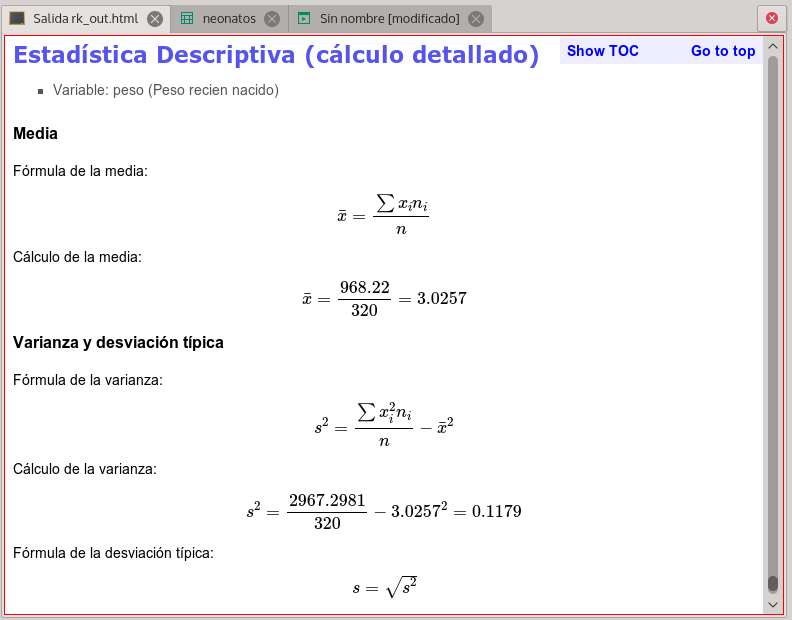
\includegraphics[width=\textwidth]{img/calculo_detallado.png}
  \caption{Salida de RKTeaching con el cálculo detallado de la media y la varianza.}
  \label{g:calculo_detallado}
\end{center}
\end{figure}

\item[Apoyo a la docencia] El paquete aporta menús y cuadros de diálogo para realizar los
procedimientos estadísticos más habituales a nivel de usuario no experto en estadística, tanto de Estadística Descriptiva como de
Estadística Inferencial (test paramétricos y no paramétricos).
Estos procedimientos son los que se suelen enseñar en las asignaturas de Estadística Aplicada en titulaciones biosanitarias.
Por tanto, el paquete es un complemento perfecto para las clases de teoría, aportando incluso simulaciones para entender algunas leyes
teóricas como la ley de los grandes números, la ley de los casos raros, el teorema central del límite o la relación entre el tamaño
muestral, la precisión y el nivel de confianza de un intervalo de confianza.
En el anexo \ref{menus_rkteaching} se muestran los menús que incorpora la versión 1.2 del paquete RKTeaching.
\end{description}

\section{Uso del paquete RKTeaching en la enseñanza de Bioestadística}
El paquete RKTeaching se ha utilizado durante los últimos cinco años para impartir las prácticas de Bioestadística en las titulaciones de
grado en Farmacia y Medicina de la Universidad CEU San Pablo. 
Para ello se ha elaborado el libro electrónico Bioestadística Aplicada con R y RKTeaching [Sánchez-Alberca A. (2014)] donde se pone
de manifiesto cómo el paquete da soporte más que suficiente a un curso básico de Estadística Aplicada a las Ciencias Biosanitarias, con
multitud de ejemplos prácticos desarrollados paso a paso. 
Es más, gracias al paquete RKTeaching, también se han podido realizar prácticas de probabilidad con experimentos aleatorios, ya que el
paquete permite construir espacios probabilísticos asociados a experimentos aleatorios y calcular probabilidades en dichos espacios, algo
que no permitía ninguno de los programas utilizados hasta la fecha.
Además el paquete incluye los conjuntos de datos necesarios para
realizar prácticamente todos los ejercicios incluidos en el libro, por lo que los alumnos no pierden tiempo en la tediosa tarea de introducir los datos de las muestras.

En los dos últimos años, el paquete RKTeaching también ha empezado a utilizarse en otras universidades, entre las que se encuentra la
Universidad Complutense, la Universidad Carlos III y la Universidad Rey Juan Carlos de Madrid.
En casi todos los casos se han interesado por el
paquete como sustituto a SPSS en las prácticas de Estadística de distintas asignaturas.

Finalmente, el paquete también se ha utilizado en un curso en línea abierto masivo (MOOC) de Bioestadística impartido en
la plataforma Miríada X [Sánchez-Alberca A. (2013)]. Se han realizado ya tres ediciones de este curso con más de 5000
alumnos de todo el mundo que ya han utilizado el paquete con una valoración por parte de los alumnos muy satisfactoria.

Finalmente, el paquete fue presentado en 2013 mediante una comunicación oral en el congreso Use R!, que es la
conferencia internacional de usuarios de R más importante del mundo. 
  

\section{Comparativa docente de RKTeaching con SPSS}
Puesto que el principal objetivo que nos marcamos al desarrollar este paquete era introducir el software libre, y en particular R, en la
docencia de Estadística con una curva de aprendizaje igual o incluso más suave que la del software utilizado hasta entonces, que
fundamentalmente era SPSS, se realizó un estudio comparativo de la facilidad de uso y el tiempo de aprendizaje entre RKTeaching y SPSS.

En el estudio se tomó una muestra de 40 alumnos de medicina que habían aprobado el curso básico de estadística pero nunca habían manejado R
con el paquete RKTeaching ni SPSS. 
Los alumnos recibieron una pequeña clase introductoria sobre la entrada de datos con cada uno de los
programas y a continuación se les pidió que realizasen una serie de ejercicios con ambos programas.
Los ejercicios consistieron en introducir los datos de una muestra, dibujar un histograma, calcular varios estadísticos descriptivos,
calcular un modelo de regresión lineal y dibujarlo, calcular una probabilidad de una variable normal y hacer un contraste de hipótesis de
comparación de medias.

Para que el orden de los programas no influyese, los alumnos se dividieron aleatoriamente en dos grupos de 20 alumnos,
de manera que los primeros empezaron con RKTeaching y luego con SPSS y los segundos al revés.
Al final, se midió el tiempo que tardaron en hacer la tarea con cada programa y también se les pidió que hicieran una
valoración sobre la facilidad de uso de cada uno de ellos.
Las variables medidas fueron: Tiempo de realización de la tarea con RKTeaching (en min), tiempo de realización de la
tarea con SPSS (en min), facilidad de uso de RKTeaching (escala discreta de 1=más difícil a 5=más fácil) y facilidad de
uso de SPSS (escala discreta de 1=más difícil a 5=más fácil).

La comparativa de los tiempos de aprendizaje mostró que el tiempo de aprendizaje de SPSS fue significativamente mayor que el tiempo de
aprendizaje con RKTeaching (ver figura~\ref{g:tiempo_aprendizaje}) con un p-valor  $4.8\cdot 10^{-17}$ y un intervalo de
confianza del 95\% para diferencia de medias $(9.06, \infty)$, lo que indica que el tiempo medio para realizar las tareas con SPSS fue al menos 9 minutos mayor que el de
RKTeaching, lo que supone una reducción del tiempo de al menos un 17\%.

\begin{figure}[htp]
\begin{center}
  \includegraphics[width=0.8\textwidth]{img/histograma_tiempo_aprendizaje.png}
  \caption{Comparativa del tiempo requerido para realizar los ejercicios del experimento con SPSS y con RKTeaching. Como se aprecia la
  distribución de tiempos con RKTeaching es claramente inferior a la de SPSS.}
  \label{g:tiempo_aprendizaje}
\end{center}
\end{figure}

De igual modo, la comparativa de la facilidad de uso reveló que la facilidad de uso de RKTeaching fue significativamente mayor que la de
SPSS (fig.\ref{g:facilidad_uso}) con un p-valor $1.7\cdot 10^{-06}$ y un intervalo de confianza del 95\% para diferencia de medias $(0.4993,
\infty)$, lo que indica que la facilidad de manejo de RKTeaching es de al menos medio punto más que con SPSS, lo que supone un aumento de la facilidad
de al menos un 10\%.

\begin{figure}[htp]
\begin{center}
  \includegraphics[width=0.8\textwidth]{img/diagrama_barras_facilidad_uso.png}
  \caption{Comparativa de la facilidad de uso de SPSS y RKTeaching. Como se
  aprecia la distribución de la puntuación de facilidad de uso de RKTeaching es claramente superior a la de SPSS.}
  \label{g:facilidad_uso}
\end{center}
\end{figure}

\section{Conclusiones y trabajo futuro}
Con el objetivo de introducir el uso del software libre, en concreto R, en la enseñanza de la estadística se ha
desarrollado el paquete RKTeaching. Este paquete incorpora a la interfaz gráfica de usuario RKWard nuevos menús y
cuadros de diálogo para desarrollar los procedimientos estadísticos de un curso básico de Estadística, de forma sencilla
e intuitiva, sin necesidad de conocer el lenguaje de programación de R.
El paquete RKTeaching se ha utilizado con éxito para impartir las prácticas de Estadística en las titulaciones de
Medicina, Farmacia y Psicología en la Universidad CEU San Pablo y en otras universidades, y también para impartir un
curso en línea abierto masivo.
Para valorar la facilidad de uso de RKTeaching frente al SPSS, que era el software utilizado hasta el momento, se
realizó un experimento que reveló que el aprendizaje con RKTeaching por parte de los alumnos es más rápido e intuitivo
que con SPSS.

Como trabajo futuro se plantea incorporar cuadros de diálogos para análisis más complejos como el análisis multivariante y mejorar aún más
la interpretación de los resultados de los análisis. 
También se ha empezado a desarrollar un módulo para la creación de ejercicios y prácticas personalizadas que permita la generación de datos
propios para cada alumno y automatice la corrección de los ejercicios planteados sobre esos datos. 

\begin{thebibliography}{9}
\bibitem{friedrichsmeier2011introduction} Friedrichsmeier T. y Michalke M. (2011). Introduction to Writting Plugins for RKWard. En:
\url{http://rkward.sourceforge.net/documents/devel/-plugins/index.html} (accedido 26 de diciembre de 2014).

\bibitem{R2001} R Development Core Team (2001). \emph{R: A Language and Environment for Statistical Computing}. Viena: R Foundation for
Statistical Computing.

\bibitem{Rödiger2012comprehensive} Rödiger S., Friedrichsmeier T., Kapat P. y Michalke M. (2012). RKWard: A Comprehensive Graphical
User Interface and Integrated Development Environment for Statistical Analysis with R. \emph{Journal of Statistical Software},
\textbf{49(9)}, 1-34.

\bibitem{sanchez2013curso} Sánchez-Alberca A. (2013). Curso Práctico de Bioestadística con R. Plataforma Miríada X. En:
\url{https://www.miriadax.net/web/curso-practico-bioestadistica-r-3edicion} (accedido 26 de diciembre de 2014).

\bibitem{sanchez2014bioestadistica} Sánchez-Alberca A. (2014). Bioestadística Aplicada con R y RKTeaching. En
\url{http://aprendeconalf.es/estadistica/bioestadistica-rkteaching} (accedido 26 de diciembre de 2014).
\end{thebibliography}

\appendix
\section*{Anexo}

\section*{Menús y procedimientos estadísticos del paquete RKTeaching}\label{menus_rkteaching}
A continuación se presenta la lista de menús y los correspondientes procedimientos estadísticos que incorpora paquete RKTeaching en su
versión 1.2.
Estos menús cuelgan de un nuevo menú \textsf{Teaching} que aparece en la barra de menús principal de RKWard tras instalar el paquete.

\setlist{noitemsep}
\setlist[itemize]{leftmargin=*}
\setlist[itemize,1]{label=$\triangleright$}
\setlist[itemize,2]{label=$\triangleright$}
\setlist[description]{leftmargin=*,font=\sffamily\bfseries}
\newcommand\litem[1]{\item{\sffamily\bfseries #1 \enspace}}

\begin{description}
\item[Datos] Manipulación y transformación de los datos de las muestras. 
\begin{itemize}
\litem {Filtrar datos} Permite seleccionar el subconjunto de individuos de la muestra que cumplen una determinada condición. 
\litem {Calcular variable} Permite calcular una nueva variable a partir de otras variables ya existentes mediante la aplicación de una
fórmula.  
\litem {Recodificar variable} Permite calcular una nueva variable a partir de otra variable ya existente definiendo rangos o intervalos de
valores en esta y asociando nuevos valores a cada rango.  
\litem {Ponderar datos} Genera un nuevo conjunto de datos a partir de los valores de las variables y las frecuencias asociadas a cada caso.
En el conjunto de datos resultantes cada caso se replica el número de veces que indica su frecuencia. 
\litem {Tipificar variables} Aplica la transformación de tipificación (restar la media y dividir por la desviación típica) a cada variable
de la muestra para obtener nuevas variables con las puntuaciones típicas de cada individuo. 
\end{itemize}

\item[Distribución de frecuencias] Tabulación y cálculo de frecuencias muestrales.
\begin{itemize}
\litem{Tabla de frecuencias} Construye la tabla de frecuencias de una variable incluyendo la frecuencia absoluta, la frecuencia relativa,
la frecuencia absoluta acumulada y la frecuencia relativa acumulada.
Permite agrupar los datos de las variables cuantitativas en intervalos. 
\litem{Tabla de frecuencias bidimensional} Construye la tabla de frecuencias absolutas o relativas de un par de variables.
Permite agrupar los datos de las variables cuantitativas en intervalos. 
\end{itemize}

\item[Gráficos] Dibujo de gráficos descriptivos.
\begin{itemize}
\litem{Diagrama de barras} Dibuja el diagrama de barras de frecuencias absolutas, relativas, absolutas acumuladas o relativas acumuladas de
una variable, así como el polígono de frecuencias asociado. 
Permite dividir la muestra en subgrupos de acuerdo a una o más variables categóricas o factores y dibujar barras diferenciadas para cada
grupo.
\litem{Histograma} Dibuja el histograma de barras de frecuencias absolutas, relativas, absolutas acumuladas o relativas acumuladas de
una variable, así como el polígono de frecuencias asociado. 
Permite dividir la muestra en subgrupos de acuerdo a una o más variables categóricas o factores y dibujar barras diferenciadas para cada
grupo.
\litem{Diagrama de sectores} Dibuja el diagrama de sectores de frecuencias absolutas o relativas de una variable.
Permite dividir la muestra en subgrupos de acuerdo a una o más variables categóricas o factores y dibujar diagramas diferenciados para cada
grupo.
\litem{Diagrama de caja} Dibuja el diagrama de caja y bigotes una o más variables cuantitativas. 
Permite dividir la muestra en subgrupos de acuerdo a una o más variables categóricas o factores y dibujar cajas diferenciadas para cada
grupo.
\litem{Diagrama de medias} Dibuja la media de una o más variables cuantitativas así como el intervalo de confianza asociado.  
Permite dividir la muestra en subgrupos de acuerdo a una o más variables categóricas o factores y dibujar medias e intervalos de confianza
diferenciados para cada grupo.
\litem{Diagrama de interacción} Dibuja las medias de una variable cuantitativa en los grupos que resultan de cruzar dos variables
categóricas o factores. 
\litem{Diagrama de dispersión} Dibuja el diagrama de dispersión de dos variables cuantitativas así como el modelo de
regresión (lineal, cuadrático, cúbico, exponencial, logarítmico, potencial, inverso o sigmoidal) asociado. 
Permite dividir la muestra en subgrupos de acuerdo a una o más variables categóricas o factores y dibujar puntos y modelos de regresión 
diferenciados para cada grupo.
\litem{Matriz de dispersión} Dibuja los diagramas de dispersión de todos los posibles pares de un conjunto de dos o más variables
cuantitativas, organizándolo en forma de matriz. Permite dibujar la recta de regresión sobre los diagramas.
\end{itemize}

\item[Estadística descriptiva] Cálculo de los estadísticos descriptivos muestrales
\begin{itemize}
\litem{Estadísticos} Calcula los estadísticos descriptivos de una o más variables cuantitativas (mínimo, máximo, media, mediana, moda,
varianza, desviación típica, cuasivarianza, cuasidesviación típica, coeficiente de variación, coeficiente de asimetría, coeficiente de
apuntamiento, cuartiles y percentiles).
Permite dividir la muestra en subgrupos de acuerdo a una o más variables categóricas o factores y calcular los estadísticos para cada
subgrupo.
\litem{Cálculo detallado} Calcula los estadísticos descriptivos más importantes de una variable cuantitativa (media, varianza, desviación
típica coeficiente de variación, coeficiente de asimetría y coeficiente de apuntamiento) mostrando la fórmulas y los todos los detalles de
cálculo. 
\end{itemize}

\item[Regresión] Construcción de modelos de regresión y correlación.
\begin{itemize}
\litem{Regresión lineal} Construye la recta de regresión de una variable cuantitativa con respecto a otra. 
\litem{Regresión no lineal} Construye el modelo de regresión (cuadrático, cúbico, exponencial, logarítmico, potencial, inverso o sigmoidal)
de regresión de una variable cuantitativa con respecto a otra.
\litem{Comparación de modelos} Calcula el coeficiente de determinación de los modelos de regresión (cuadrático, cúbico, exponencial,
logarítmico, potencial, inverso o sigmoidal) de una variable cuantitativa con respecto a otra y los ordena de mayor a menor. 
\litem{Predicciones} Permite hacer predicciones de la variable dependiente mediante un modelo de regresión dado y uno o varios valores de la
variable independiente.  
\litem{Correlación} Calcula la matriz de correlación (Person, Kendall o Spearman) de dos o más variables cuantitativas. 
\end{itemize}

\item[Test paramétricos] Estimación y contrastes de hipótesis poblacionales paramétricos 
\begin{description}
\item[Medias]\mbox{}\\[-1\baselineskip]
\begin{itemize}
\litem{Test T para una muestra} Permite realizar el contraste de la T de Student sobre la media poblacional de una variable cuantitativa y
estimarla mediante un intervalo de confianza. 
\litem{Test T para dos muestras independientes} Permite realizar el contraste de la T de Student para ver si hay diferencias significativas
entre las medias poblacionales de una variable cuantitativa en dos poblaciones distintas y estimar cuánto vale la diferencia entre las medias mediante un
intervalo de confianza. 
\litem{Test T para dos muestras pareadas} Permite realizar el contraste de la T de Student para ver si hay diferencias significativas entre
las medias poblacionales de dos variables cuantitativas medidas en la misma población y estimar cuánto vale la diferencia entre las medias mediante un
intervalo de confianza. 
\litem{ANOVA} Permite realizar el contraste de Análisis de la Varianza para ver si hay diferencias significativas entre las medias
poblacionales de una variable cuantitativa en dos o más poblaciones, así como hacer los contrastes de comparación por pares de Tukey. 
\litem{Cálculo del tamaño muestral para la media} Permite calcular el tamaño muestral necesario para estimar la media poblacional de una
variable cuantitativa con una precisión y una confianza dadas. 
\litem{Cálculo del tamaño muestral para el test T} Permite calcular el tamaño muestral necesario para determinar una diferencia igual o
superior a una dada entre las medias poblacionales de una variable cuantitativa con un nivel de significación y una potencias dados. 
\end{itemize}

\item[Varianzas]\hfill\\[-1\baselineskip]
\begin{itemize}
\litem{Test F de Fisher} Permite realizar el contraste de la F de Fisher para ver si hay diferencias significativas entre las varianzas
poblacionales de una variable cuantitativa en dos poblaciones distintas y estimar cuánto vale el cociente entre varianzas mediante un intervalo de confianza.  
\litem{Test de Levene} Permite realizar el contraste de Levene para ver si hay diferencias significativas entre las varianzas (medidas con
respecto a la media o a la mediana) poblacionales de una variable cuantitativa en dos o más poblaciones distintas y estimar cuánto vale el cociente
entre varianzas mediante un intervalo de confianza.
\end{itemize}

\item[Proporciones]\hfill\\[-1\baselineskip]
\begin{itemize}
\litem{Test para una proporción} Permite realizar un contraste sobre la proporción poblacional de individuos que presentan un determinado
valor en una variable cualitativa o factor y estimarla mediante un intervalo de confianza.
\litem{Test para dos proporciones} Permite
realizar un contraste para ver si hay diferencias significativas entre las proporciones poblacionales de invidivudos que presentan un determinado valor en una variable categórica o factor en dos poblaciones distintas y estimar
cuánto vale la diferencia entre las proporciones mediante un intervalo de confianza. 
\litem{Cálculo del tamaño muestral para una proporción} Permite calcular el tamaño muestral necesario para estimar la proporción 
poblacional de individuos que presentan un determinado valor en una variable categórica o factor con una precisión y una confianza dadas. 
\end{itemize}
\end{description}

\item[Test no paramétricos] Contrastes de hipótesis poblacionales no paramétricos
\begin{description}
\item[Normalidad]\hfill\\[-1\baselineskip]
\begin{itemize}
\litem{Test de Lilliefors (Kolmogorov-Smirnov)} Permite realizar el contraste de Lilliefors (corrección del test de Kolmogorov-Smirnov) para
ver si una variable tiene distribución normal. 
\litem{Test de Shapiro-Wilk} Permite realizar el contraste de Shapiro-Wilk para ver si una variable tiene
distribución normal. 
\end{itemize}
\end{description}
\begin{itemize}
\litem{Test U de Mann-Whitney para dos muestras independientes} Permite realizar el contraste de la U de Mann-Whitney para ver si existen
diferencias significativas en las distribuciones de probabilidad de una variable ordinal medida en dos poblaciones independientes.   
\litem{Test de Wilcoxon para dos muestras pareadas} Permite realizar el contraste de Wilcoxon para ver si existen
diferencias significativas en las distribuciones de probabilidad de dos variables ordinales medidas en la misma población. 
\litem{Test de Kruskal-Wallis para varias muestras independientes} Permite realizar el contraste de Kruskal-Wallis para ver si existen
diferencias significativas en las distribuciones de probabilidad de una variable ordinal medida en dos o más poblaciones independientes.
\litem{Test de Friedman para medidas repetidas} Permite realizar el contraste de Friedman para ver si existen
diferencias significativas en las distribuciones de probabilidad de dos o más variables ordinales medidas en la misma población. 
\litem{Test Chi-cuadrado de independencia} Permite realizar el contraste de la Chi-cuadrado para ver si existe relación significativa entre
dos variables cualitativas medidas en una misma población. 
\litem{Test Chi-cuadrado de bondad de ajuste} Permite realizar el contraste de la Chi-cuadrado para ver las frecuencias muestrales de una
variable se ajustan a una distribución de probabilidad dada. 
\end{itemize}

\item[Concordancia] Estudio de la concordancia o acuerdo entre dos variables. 
\begin{itemize}
\litem{Coeficiente de correlación intraclase} Calcula el coeficiente de correlación intraclase para ver si existe concordancia o acuerdo
entre dos variables cuantitativas. 
\litem{Kappa de Cohen} Calcula el coeficiente kappa de Cohen para ver si existe concordancia o acuerdo entre dos variables cualitativas.  
\end{itemize}

\item[Probabilidad] Definición de espacios probabilísticos de experimentos aleatorios y cálculo de probabilidades. 
\begin{description}
\item[Juegos de azar] \hfill\\[-1\baselineskip] 
\begin{itemize}
\litem{Monedas} Permite construir el espacio probabilístico del experimento aleatorio consistente en lanzar varias monedas un número
determinado de veces, así como simular dicho experimento. 
\litem{Dados}  Permite construir el espacio probabilístico del experimento aleatorio consistente en lanzar varios dados un número
determinado de veces, así como simular dicho experimento. 
\litem{Naipes} Permite construir el espacio probabilístico del experimento aleatorio consistente en sacar varias cartas de una baraja de
naipes, así como simular dicho experimento. 
\litem{Urnas}  Permite construir el espacio probabilístico del experimento aleatorio consistente en sacar varios objetos de una urna con o
sin reemplazamiento, así como simular dicho experimento.
\end{itemize}
\end{description}
\begin{itemize}
\litem{Construcción de espacio probabilístico} Permite construir un espacio probabilístico a partir de los casos de una muestra y sus
frecuencias relativas. 
\litem{Combinación de espacios probabilísticos} Permite construir un espacio probabilístico a partir de la combinación varios espacios
probabilísticos independientes. 
\litem{Repetición de espacios probabilísticos} Permite construir un espacio probabilístico replicando otro espacio probabilístico dado un
número de veces determinado. 
\litem{Cálculo de probabilidad} Permite calcular la probabilidad de un suceso en un espacio probabilístico dado o la probabilidad de ese
suceso condicionada por otro dado. 
\end{itemize}

\item[Distribuciones de probabilidad] Cálculo de probabilidades con modelos de distribución de probabilidad clásicos. 
\begin{description}
\item[Distribuciones discretas] \hfill\\[-1\baselineskip] 
\begin{itemize}
\litem{Binomial} Permite calcular probabilidades, probabilidades acumuladas y cuantiles con un modelo de distribución Binomial, así como
dibujar su función de probabilidad o de distribución.
\litem{Poisson} Permite calcular probabilidades, probabilidades acumuladas y cuantiles con un modelo de distribución de Poisson, así como
dibujar su función de probabilidad o de distribución.
\end{itemize}
\item[Distribuciones continuas] \hfill\\[-1\baselineskip] 
\begin{itemize} 
\litem{Chi-cuadrado} Permite calcular probabilidades acumuladas y cuantiles con un modelo de distribución Chi-cuadrado, así como
dibujar su función de probabilidad o de distribución.
\litem{F de Fisher} Permite calcular probabilidades acumuladas y cuantiles con un modelo de distribución F de Fisher, así como
dibujar su función de probabilidad o de distribución.
\litem{Normal} Permite calcular probabilidades acumuladas y cuantiles con un modelo de distribución Normal, así como
dibujar su función de probabilidad o de distribución.
\litem{T de student} Permite calcular probabilidades acumuladas y cuantiles con un modelo de distribución T de student, así como
dibujar su función de probabilidad o de distribución.
\litem{Uniforme continua} Permite calcular probabilidades acumuladas y cuantiles con un modelo de distribución Uniforme, así como
dibujar su función de probabilidad o de distribución.
\end{itemize}
\end{description}

\item[Simulaciones] Simulaciones interactivas de varias leyes. 
\begin{itemize}
\litem{Ley de los casos raros} Realiza una simulación de la aproximación de una distribución Binomial mediante una
distribución de Poisson permitiendo que el usuario varíe los parámetros de la Binomial. 
\litem{Teorema central del límite} Realiza una simulación del Teorema Central del Límite generando varias variables con
distribuciones fijadas por el usuario y dibujando la distribución de la suma.
\litem{Precisión de un intervalo de confianza} Muestra un gráfico que refleja cómo varía la precisión de un intervalo de confianza a medida
que cambiamos el tamaño de la muestra o el nivel de confianza del intervalo. 
\end{itemize}
\end{description}


\subsection*{Acerca de los autores}%

\textbf{Alfredo Sánchez Alberca} es profesor de Matemáticas en el Departamento de Matemática Aplicada y Estadística de la Universidad
CEU San Pablo de Madrid. Es también miembro de la Unidad de Bioestadística de la Universidad CEU San Pablo donde ha
dirigido multitud de estudios clínicos y epidemiológicos. Sus principales áreas de investigación son la Estadística
Aplicada y la Inteligencia Artificial, así como la docencia de Matemáticas y Estadística. 

\end{document}
